% chap3.tex


\chapter{Visibility Driven Transfer function}\label{chap:ch4_abbr}

\section{Motivation}

Medical imaging has given radiologists an ability that photography was not able to provide, it lets them see inside the human body. With the advent of 3D visualization systems, these images can be put together into crisp and impressive renderings of the human body from a variety of perspectives that were only dreamt of before, revolutionizing clinical practice.

Light transport models soon emerged to allow light interactions that, although not realistic in the physical sense, proved to be more effective for understanding the complex relationships among the anatomical structures. For instance, bone could be made semi-transparent to provide visibility of brain tissue. Skin could be removed altogether from an image to show only muscle or internal organs. However, soon it
became evident that simply rendering these images in their raw form was no longer effective and the clear visualization of internal structures remains elusive.

The depiction of internal parts in the context of the enclosing space is a difficult problem that has occupied the mind of artists, illustrators and visualization practitioners. Despite the advances made in computer graphics for simulating the light transport in semi-transparent media, the problem of visualizing internal objects is no longer a rendering problem, but that of classification. Medical imaging technology obtains representations of anatomical structures via indirect ways, such as the response of tissue to X-rays or the alignment of electrons in a magnetic field. Therefore, the absence of semantic information prevents visualization practitioners from clearly marking up the regions that must be visualized. Without access to those regions, exploration becomes tedious and time-consuming. The predominant approach has been the use of transfer functions, or opacity mappings, which assign transparency properties to different intervals in the data. This method, however, does not guarantee visibility that internal structures or structures of interest in the volume. There is need to incorporate a measure for visibility. In this chapter, visualization techniques to obtain clear views of internal features in 3D volume data is discussed along with visibility metric.

\section{Related Work}

With the fast growth in computational power of graphics hardware, only until recently it has been possible to manipulate 3D volume data in fashions that were only possible for surface meshes and CAD models, where semantic information is often explicit and readily available. When volume data are understood as explorable objects, we can disassemble it into parts that can be decomposed in numerous ways. One of the foremost ideas that were explored in this direction where cutaways, where certain parts can be removed to uncover hidden parts of the 3D volume. [14] Exploded views extend this idea to reveal the relationships among the internal parts of a complex volume [1].

Another strategy is to assign material properties to different regions or layers of a volume and simulate the physical response to the deformation and cutting of such regions [5,6,10]. 

Although the deformation “unrealistically” simulates an elastic material for the piggy bank, the metaphor is effective for depicting the internal structures. More realistic effects are obtained by simulating the response of tissue, such as skin, to incisions and retractions, as used in real surgical procedures. Figure 3 shows the result of peeling the skin, and muscle layers of a foot CT scan to reveal the internal vessels (left) or bone (right).

Rigid and deformable cuts, although effective for visualizing the internal structures, work under the premise that the internal and external layers are clearly separated. In a more general sense, this separation is not easy to come by, and, in most cases, there is a degree of uncertainty. For this reason, the effective visualization of internal structure must rely on robust classification.

The main challenge when attempting to see the internal features remains that of classification. An effective visualization must first decide what is it that we must preserve and what regions are unimportant. Traditional classification systems, found in off-the-shelf visualization systems, only consider a single dimension for classification, without regards of the spatial characteristics or the semantics of the data. However, volume data seldom contain any semantics about the captured structures. Acquisition technology outputs a series of images with intensity values, while simulations of 3D phenomena sample a continuous scalar or vector field in a grid.

In an attempt to extract semantic information, one may analyze the spatial properties of the data, such as the location of boundaries [9], regions of high curvature [7], shape [12] or size[6]. In most of these cases, these properties are just approximations of the local distribution of data in a small neighborhood. Size, for example, can be measured as the extents of regions of a certain homogeneity. Regions of a certain material, such as brain, that occupy a large volume, have different properties than those regions, such as skull and
skin, that are relatively thin.

These observations have enabled us to construct classification based on size, and assign opacity based on the relative thickness of features. A particular example is the visualization of brain MRI, where the data is comprised of a series of thin layers (i.e, skin, skull and tissue) surrounding a large region, the brain, of a certain material. Exploiting these properties lets us minimize the effects of occluding tissue, such as skin, to reveal the brain tissue clearly, as shown in Figure 4.

Other approaches do not operate on the data itself but on the rendering process. For example, importance-driven techniques [13] and ghosted views [2,8] assign different opacities in a viewpoint dependent manner, so that the user constantly gets an uninterrupted view of internal structures. A different approach, opacity peeling, automatically finds the layers that compose an image from a given point of view [11].

\section{Notion of Visibility metric} 

One of the limitations of contemporary visualization systems is the inability to quantify how visible a feature of interest is. To be more effective, along with traditional transfer function design, must incorporate a measure of visibility. 

Visibility Metric attemps to measure the impact of individual samples on the image generated by a volumetric object. It is measured as the contribution of a structure of interest to the final image. Here, visibility can be used to quantify the quality of transfer function and ease their design towards more meaningful and efficient visualization. Transfer function generated with this approach are called as visibility driven transer functions.

This process measures visibility of all structures in a volume to arrive at a good transfer function. In general, a visibility-driven transfer function is constructed in such a way that we guarantee the visibility of all structures of interest and at the same time maximizes the visibility of structure of interest, in particular, of those features lying at the interior of a data set. 


\section{Visibility Histogram}

The contribution of a sample in the volume to final image is refered to as visibility of that sample. 


$ \alpha (s) \; = \; 1 \; - \; e^{\int^{D}_{s} \tau(t) dt \; } $   .....(3.1)


where $ \tau(t) $ is the attenuation coefficient of a sample, usually represented as an opacity transfer function $\mathcal{O}$ which is defined by user. Visibility also depends viewpoint as accumulated opacity in front of the sample may differ at different viewpoints. 

A visibility histogram is a graphical representation of distribution of visibility function in relation to the domain values of the volume. Samples are weighted by visibility and added into bins that partition the range of values in the scalar field. 

VH(x) = $ \mathcal{O} (x) \int_{s \epsilon \omega} \delta(s, x) (1 \; - \; \alpha(s) ) ds $  .....(3.2)
where, $ \delta(s, x) $ is a function.


\[
    \delta(s, x)=\left\{
                \begin{array}{ll}
                  1  \;\;\;\;\;\;\;    V(s) = x\\
                  0  \;\;\;\;\;\;\;    Otherwise \;\;\;\;\;\;\; .....(3.2)\\
                \end{array}
              \right.
\]



In this thesis, front-to-back compositing is used, as discussed in section 2.4.3. Accumulated opacity is computed as, 


AccumulatedOpacity[i] = AccumulatedOpacity[i-1] + ( 1 - AccumulatedOpacity ) Opacity(x) 

Hence, for all sample values x in the volume.
VH[x] = VH[x] + ( 1 - AccumulatedOpacity ) Opacity(x)

\begin{figure}
\centering
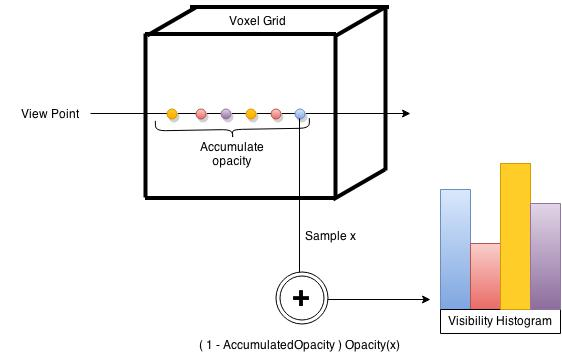
\includegraphics[width=350pt]{Images/VHistogram.jpg}
\caption{\label{fig:ray_cast1.jpg} Direct Volume rendering using Raycasting.}
\end{figure}


Visibility histogram helps find string occusion patterns on the data, as shown in the figure 3.1. 


\begin{figure}
\centering
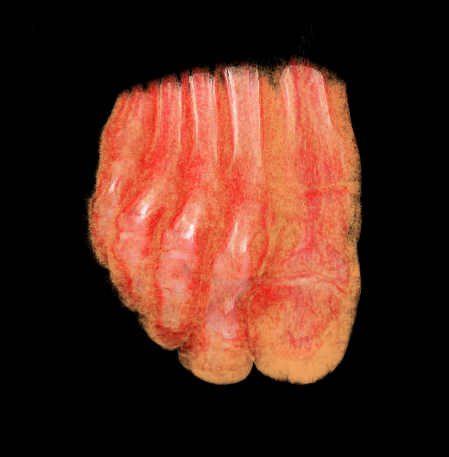
\includegraphics[width=150pt]{Images/foot_1.png}
\caption{\label{fig:ray_cast1.jpg} Direct Volume rendering using Raycasting.}
\end{figure}






   

